% Source: StudentGovernmentRepo/Common_Sense_Carolina_Lobbying_org/figures/org_phase3.tex
\documentclass[border=5pt]{standalone}
\usepackage{tikz}
\usepackage{xcolor}
\usetikzlibrary{arrows.meta}

\definecolor{garnet}{HTML}{73000A}
\definecolor{rose}{HTML}{CC2E40}
\definecolor{atlantic}{HTML}{466A9F}
\definecolor{congaree}{HTML}{1F414D}
\definecolor{horseshoe}{HTML}{65780B}
\definecolor{warmgrey}{HTML}{676156}
\definecolor{sandstorm}{HTML}{FFF2E3}

\begin{document}
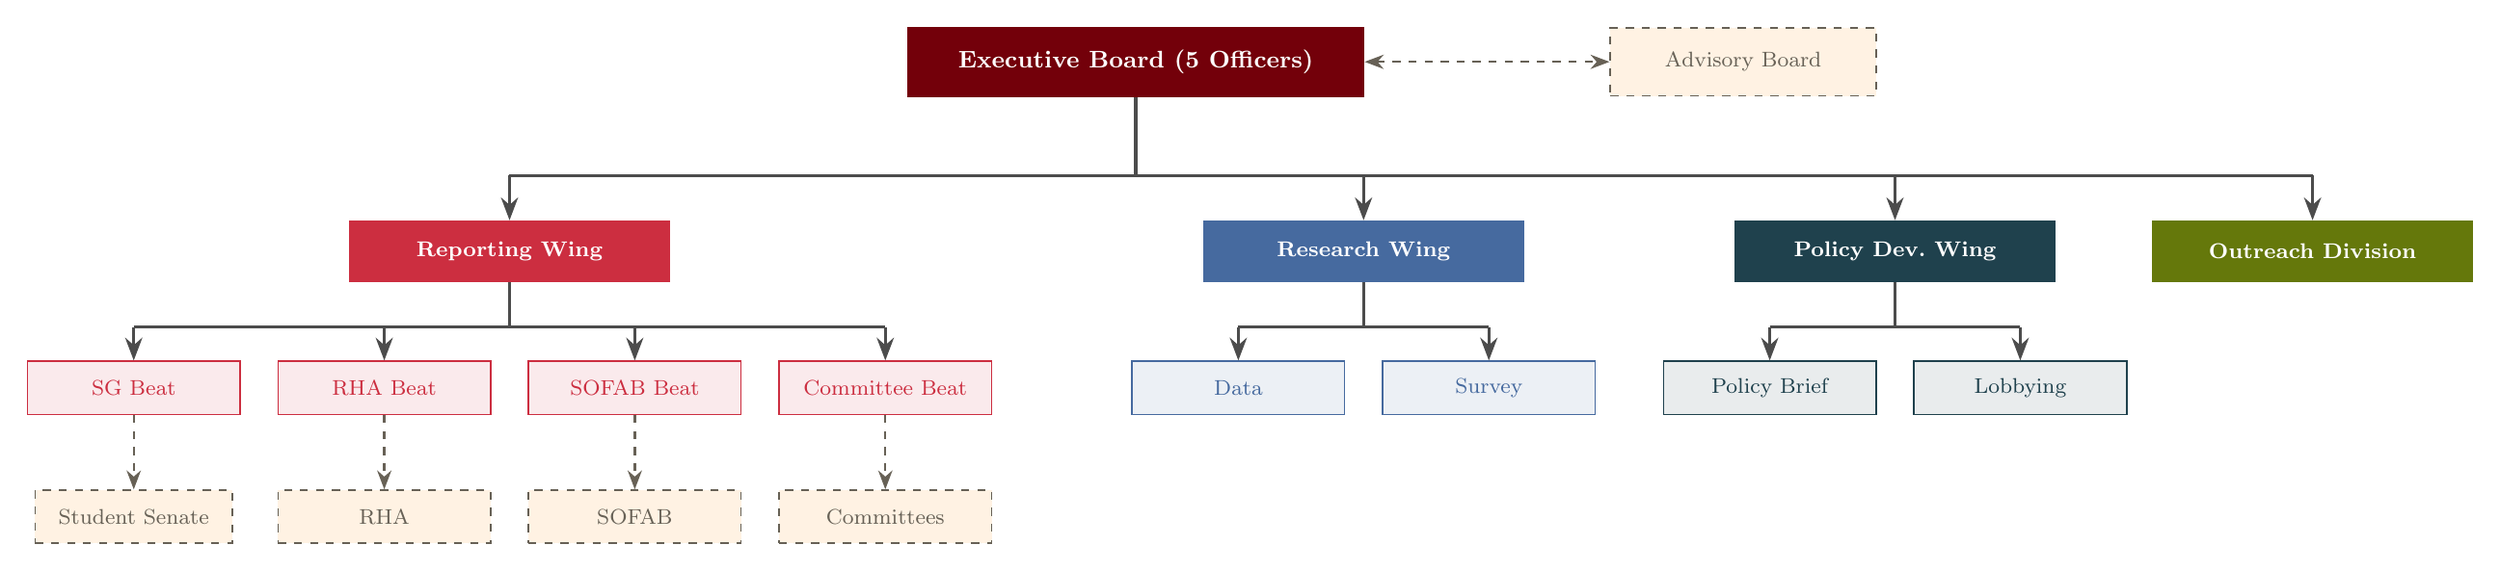
\begin{tikzpicture}[
  every node/.style={rectangle, sharp corners, align=center},
  arrow/.style={-{Stealth[length=3mm]}, line width=1.2pt, black!70},
  dasharrow/.style={-{Stealth[length=2.5mm]}, line width=0.8pt, dashed, warmgrey}
]

%% Row 0: Executive Board + Advisory Board
\node[
  fill=garnet, text=white, draw=garnet, line width=0.8pt,
  font=\small\bfseries,
  minimum width=6cm, minimum height=0.9cm
] (exec) at (0,0) {Executive Board (5 Officers)};

\node[
  fill=sandstorm, draw=warmgrey, line width=0.6pt, dashed,
  font=\footnotesize, text=warmgrey,
  minimum width=3.5cm, minimum height=0.9cm
] (advisory) at (8,0) {Advisory Board};

\draw[line width=0.8pt, dashed, warmgrey, {Stealth[length=2.5mm]}-{Stealth[length=2.5mm]}]
  (exec.east) -- (advisory.west);

%% Row 1: Wings
\node[
  fill=rose, text=white, draw=rose, line width=0.6pt,
  font=\footnotesize\bfseries,
  minimum width=4.2cm, minimum height=0.8cm
] (rep) at (-8.25,-2.5) {Reporting Wing};

\node[
  fill=atlantic, text=white, draw=atlantic, line width=0.6pt,
  font=\footnotesize\bfseries,
  minimum width=4.2cm, minimum height=0.8cm
] (res) at (3,-2.5) {Research Wing};

\node[
  fill=congaree, text=white, draw=congaree, line width=0.6pt,
  font=\footnotesize\bfseries,
  minimum width=4.2cm, minimum height=0.8cm
] (pol) at (10,-2.5) {Policy Dev.\ Wing};

\node[
  fill=horseshoe, text=white, draw=horseshoe, line width=0.6pt,
  font=\footnotesize\bfseries,
  minimum width=4.2cm, minimum height=0.8cm
] (out) at (15.5,-2.5) {Outreach Division};

%% T-junction: Exec to Wings
\draw[line width=1.2pt, black!70] (exec.south) -- (0,-1.5);
\draw[line width=1.2pt, black!70] (-8.25,-1.5) -- (15.5,-1.5);
\draw[arrow] (-8.25,-1.5) -- (rep.north);
\draw[arrow] (3,-1.5) -- (res.north);
\draw[arrow] (10,-1.5) -- (pol.north);
\draw[arrow] (15.5,-1.5) -- (out.north);

%% Row 2: Beat Teams (3cm wide, 3.3cm spacing within group, 4cm between groups)
%% Under Reporting: centered at -9, spread 3.3cm apart
\node[
  fill=rose!10, draw=rose, text=rose, line width=0.6pt,
  font=\footnotesize,
  minimum width=2.8cm, minimum height=0.7cm
] (sgbeat) at (-13.2,-4.3) {SG Beat};

\node[
  fill=rose!10, draw=rose, text=rose, line width=0.6pt,
  font=\footnotesize,
  minimum width=2.8cm, minimum height=0.7cm
] (rhabeat) at (-9.9,-4.3) {RHA Beat};

\node[
  fill=rose!10, draw=rose, text=rose, line width=0.6pt,
  font=\footnotesize,
  minimum width=2.8cm, minimum height=0.7cm
] (sofabbeat) at (-6.6,-4.3) {SOFAB Beat};

\node[
  fill=rose!10, draw=rose, text=rose, line width=0.6pt,
  font=\footnotesize,
  minimum width=2.8cm, minimum height=0.7cm
] (commbeat) at (-3.3,-4.3) {Committee Beat};

%% Under Research (centered at x=3): at 1.35 and 4.65
\node[
  fill=atlantic!10, draw=atlantic, text=atlantic, line width=0.6pt,
  font=\footnotesize,
  minimum width=2.8cm, minimum height=0.7cm
] (data) at (1.35,-4.3) {Data};

\node[
  fill=atlantic!10, draw=atlantic, text=atlantic, line width=0.6pt,
  font=\footnotesize,
  minimum width=2.8cm, minimum height=0.7cm
] (survey) at (4.65,-4.3) {Survey};

%% Under Policy (centered at x=10): at 8.35 and 11.65
\node[
  fill=congaree!10, draw=congaree, text=congaree, line width=0.6pt,
  font=\footnotesize,
  minimum width=2.8cm, minimum height=0.7cm
] (brief) at (8.35,-4.3) {Policy Brief};

\node[
  fill=congaree!10, draw=congaree, text=congaree, line width=0.6pt,
  font=\footnotesize,
  minimum width=2.8cm, minimum height=0.7cm
] (lobby) at (11.65,-4.3) {Lobbying};

%% Arrows: Wings to Beat Teams (T-junctions per wing)
%% Reporting Wing
\draw[line width=1.2pt, black!70] (rep.south) -- (-8.25,-3.5);
\draw[line width=1.2pt, black!70] (-13.2,-3.5) -- (-3.3,-3.5);
\draw[arrow] (-13.2,-3.5) -- (sgbeat.north);
\draw[arrow] (-9.9,-3.5) -- (rhabeat.north);
\draw[arrow] (-6.6,-3.5) -- (sofabbeat.north);
\draw[arrow] (-3.3,-3.5) -- (commbeat.north);

%% Research Wing (centered at x=3)
\draw[line width=1.2pt, black!70] (res.south) -- (3,-3.5);
\draw[line width=1.2pt, black!70] (1.35,-3.5) -- (4.65,-3.5);
\draw[arrow] (1.35,-3.5) -- (data.north);
\draw[arrow] (4.65,-3.5) -- (survey.north);

%% Policy Dev Wing (centered at x=10)
\draw[line width=1.2pt, black!70] (pol.south) -- (10,-3.5);
\draw[line width=1.2pt, black!70] (8.35,-3.5) -- (11.65,-3.5);
\draw[arrow] (8.35,-3.5) -- (brief.north);
\draw[arrow] (11.65,-3.5) -- (lobby.north);

%% Row 3: External Bodies (dashed — monitored orgs)
\node[
  fill=sandstorm, draw=warmgrey, line width=0.6pt, dashed,
  font=\footnotesize, text=warmgrey,
  minimum width=2.6cm, minimum height=0.7cm
] (senate) at (-13.2,-6) {Student Senate};

\node[
  fill=sandstorm, draw=warmgrey, line width=0.6pt, dashed,
  font=\footnotesize, text=warmgrey,
  minimum width=2.8cm, minimum height=0.7cm
] (rha) at (-9.9,-6) {RHA};

\node[
  fill=sandstorm, draw=warmgrey, line width=0.6pt, dashed,
  font=\footnotesize, text=warmgrey,
  minimum width=2.8cm, minimum height=0.7cm
] (sofab) at (-6.6,-6) {SOFAB};

\node[
  fill=sandstorm, draw=warmgrey, line width=0.6pt, dashed,
  font=\footnotesize, text=warmgrey,
  minimum width=2.8cm, minimum height=0.7cm
] (committees) at (-3.3,-6) {Committees};

%% Dashed arrows: Beats to External Bodies (aligned 1:1)
\draw[dasharrow] (sgbeat.south) -- (senate.north);
\draw[dasharrow] (rhabeat.south) -- (rha.north);
\draw[dasharrow] (sofabbeat.south) -- (sofab.north);
\draw[dasharrow] (commbeat.south) -- (committees.north);

\end{tikzpicture}
\end{document}
